\section{Method}

In this section we cover the precise details of how to construct the objective and constraint equations,
given that we represent $\bm{x}(t)$ as a cubic spline.

\subsection{Assumptions}

To make this problem tractable, we will make two simplifying assumptions:
\begin{itemize}
  \setlength\itemsep{0em}
  \item the trajectory will be a cubic spline
  \item the knot points of the spline will be given
\end{itemize}

\subsection{Outline}

The problem outlined in Section \ref{sec:ProblemStatement} can be posed as a quadratic program,
where $\mathcal{H}$ and $\bf{f}$ are the quadratic and linear cost matrices,
$\mathcal{A}$ and $\bf{b}$ are the equality constraints, and
$\bm{z}$ is the vector of decision variables: the coefficients of the cubic spline.

\begin{align}
  & \quad  & \quad & \quad &
    \text{minimize:}  & \quad  & \tfrac{1}{2} \bm{z}^T \mathcal{H} \bm{z} + \bm{f}^T \bm{z}
  & \quad  & \quad &  \quad &\\
  & \quad  & \quad & \quad &
    \text{subject to:}  & \quad & \mathcal{A} \bm{z} = \bm{b}
  & \quad  & \quad & \quad &
\end{align}

This is a special quadratic program: it does not have inequality constraints.
As a result, this quadratic program can be solved as the linear system shown below,
where $\bm{w}$ is a vector of Lagrange multipliers for the constraint equations.

\begin{equation}

\begin{bmatrix}
\mathcal{H} & \mathcal{A}^T \\
\mathcal{A} & \bm{0}
\end{bmatrix}
\cdot
\begin{bmatrix}
\bm{z} \\
\bm{w}
\end{bmatrix}
=
\begin{bmatrix}
-\bm{f}  \\
\bm{b}
\end{bmatrix}

\label{eqn:linearSplineSystem}
\end{equation}

Once we have constructed the matrices
$\mathcal{H}$,  $\bf{f}$,  $\mathcal{A}$, and $\bf{b}$,
we can then solve the linear system (\ref{eqn:linearSplineSystem})
for the decision variables to $\bm{z}$: the spline coefficients.

\subsection{Block Matrices}

Note that the matrices $\mathcal{H}$ and $\mathcal{A}$ are large and sparse,
as shown in Figure \ref{fig:SparsityPattern}.
These matrices should be implemented as sparse matrices, and the linear system solved using a sparse solver.

\begin{figure}[ht]
	\centering
  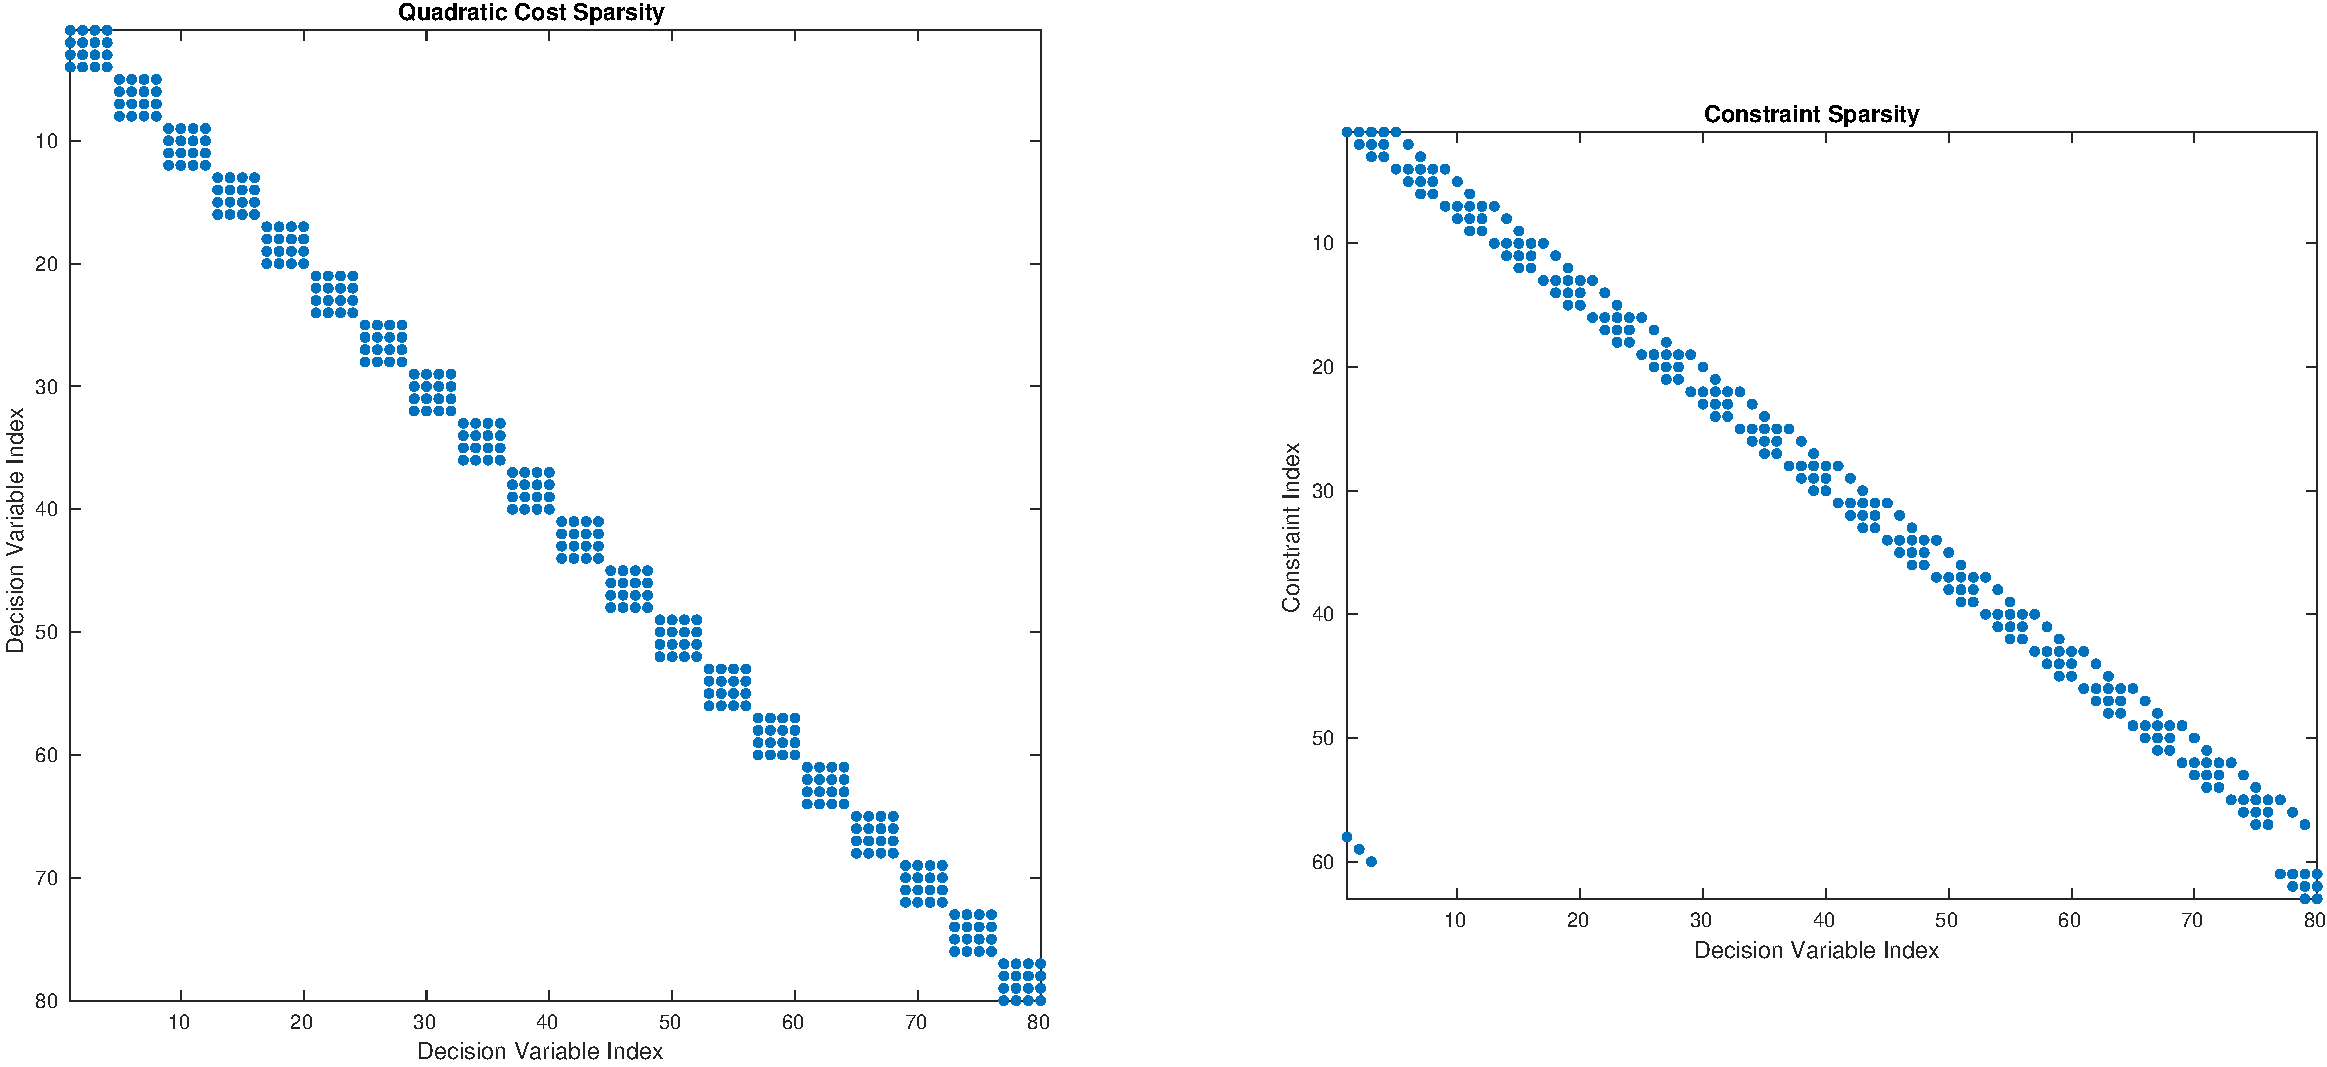
\includegraphics[width=\textwidth]{fig/SparsityPattern.pdf}
  \caption{The sparsity pattern for the spline shown in Figure \ref{fig:DataFittingExampleFigure}.
           It has 20 cubic segments and thus 4*20 = 80 decision variables.
           Notice that the quadratic cost matrix is perfectly block diagonal.
           The first 3*(20-1) rows of the constraint matrix are perfectly block diagonal,
             representing the continuity constraints.
           The final six rows are different, representing the boundary constraints.}
  \label{fig:SparsityPattern}
\end{figure}

The matrices $\mathcal{H}$ and $\mathcal{A}$ are constructed from smaller blocks,
where each block corresponds to the coefficients of a single segment. For example,
$\mathcal{H}_j$ is the $4 \times 4$ block in the $\mathcal{H}$ matrix that corresponds to the
spline segment $j$.
Similarly, $\mathcal{A}_{k,j}$ is the $3 \times 4$ block of coefficients
for the $k^\text{th}$ set of constraints on the coefficients of spline segment $j$.

\subsection{Spline Definition}

We will represent the trajectory as a cubic spline, with knot points $T_j$ where $j \in \{ 0 \dots M\}$.
A single segment of the spline is given below,
where $j$ is the segment index, and
$\tau = t - T_j$ is the time since the start of the segment.
The function $\bm{x}(t)$ is constructed by chaining together each of the segments $\bm{x}_j(t)$ in order.

\begin{equation}
  \bm{x}_j(\tau) = \bm{A}_j \tau^3 + \bm{B}_j \tau^2 + \bm{C}_j \tau + \bm{D}_j
\end{equation}

The derivatives of this spline are easily computed, as shown below:
\begin{equation}
  \dot{\bm{x}}_j(\tau)
    = \frac{d}{dt} \bm{x}_j(\tau)
    = 3 \bm{A}_j \tau^2 + 2 \bm{B}_j \tau + \bm{C}_j
\end{equation}
\begin{equation}
  \ddot{\bm{x}}_j(\tau)
    = \frac{d}{dt} \dot{\bm{x}}_j(\tau)
    = 6 \bm{A}_j \tau + 2 \bm{B}_j
\end{equation}
\begin{equation}
  \dddot{\bm{x}}_j(\tau)
    = \frac{d}{dt} \ddot{\bm{x}}_j(\tau)
    = 6 \bm{A}_j
\end{equation}

We will represent the coefficients of a single segment of the spline as
$\bm{z}_j = [\bm{D}_j, \bm{C}_j, \bm{B}_j, \bm{A}_j]^T$,
and the coefficients of the entire spline as
$\bm{z} = [\bm{z}_0, \bm{z}_1, \dots, \bm{z}_{M-1}]^T$.

%~~~~~~~~~~~~~~~~~~~~~~~~~~~~~~~~~~~~~~~~~~~~~~~~~~~~~~~~~~~~~~~~~~~~~~~~~~~~%

\subsection{Spline Continuity}

The spline coefficients are constructed such that value, slope, and curvature are continuous.
This can be written as a set of three equations at each knot point, where
$h_j = T_{j+1} - T_j$ is the duration of segment $j$.
\begin{equation}
  \bm{x}_j(h_j) - \bm{x}_{j+1}(0) = \bm{0}
\end{equation}
\begin{equation}
  \dot{\bm{x}}_j(h_j) - \dot{\bm{x}}_{j+1}(0) = \bm{0}
\end{equation}
\begin{equation}
  \ddot{\bm{x}}_j(h_j) - \ddot{\bm{x}}_{j+1}(0) = \bm{0}
\end{equation}

These equations form the blocks on the diagonals of the $\mathcal{A}$ matrix.
Each set of three constraints at a knot point populates two blocks of the constraint matrix,
one for the lower segment and one for the upper segment.


\begin{equation}
\begin{bmatrix}
\mathcal{A}_{k, j} & \mathcal{A}_{k, j+1}
\end{bmatrix}
\cdot
\begin{bmatrix}
\bm{z_j} \\
\bm{z_{j+1}}
\end{bmatrix}
=
\bm{b}_k
\label{eqn:continuityEquationsSymbols}
\end{equation}

%~~~~~~~~~~~~~~~~~~~~~~~~~~~~~~~~~~~~~~~~~~~~~~~~~~~~~~~~~~~%

\begin{equation}

\mathcal{A}_{k, j}
=
\begin{bmatrix}
1 & h_j & h_j^2  & h_j^3 \\
0 & 1   & 2 h_j  & 3 h_j^2 \\
0 & 0   & 2      & 6 h_j
\end{bmatrix}

\quad \quad \quad

\mathcal{A}_{k, j+1}
=
\begin{bmatrix}
-1 & 0 & 0  & 0 \\
0 & -1   & 0  & 0 \\
0 & 0   & -2      & 0
\end{bmatrix}

\label{eqn:continuityEquationExplicitPartOne}
\end{equation}

%~~~~~~~~~~~~~~~~~~~~~~~~~~~~~~~~~~~~~~~~~~~~~~~~~~~~~~~~~~~%

\begin{equation}

\bm{z}_j
=
\begin{bmatrix}
\bm{D}_j \\
\bm{C}_j \\
\bm{B}_j \\
\bm{A}_j
\end{bmatrix}

\quad \quad \quad

\bm{z}_{j+1}
=
\begin{bmatrix}
\bm{D}_{j+1} \\
\bm{C}_{j+1} \\
\bm{B}_{j+1} \\
\bm{A}_{j+1}
\end{bmatrix}

\quad \quad \quad

\bm{b}_k
=
\begin{bmatrix}
\bm{0} \\
\bm{0} \\
\bm{0}
\end{bmatrix}


\label{eqn:continuityEquationExplicitPartTwo}
\end{equation}


%~~~~~~~~~~~~~~~~~~~~~~~~~~~~~~~~~~~~~~~~~~~~~~~~~~~~~~~~~~~~~~~~~~~~~~~~~~~~%
\subsection{Boundary Constraints}

The boundary constraints are similar to the continuity equations,
but they use only a single block in the $\mathcal{A}$ matrix and a non-zero block in the $\bm{b}$ matrix.
To keep notation simple through this section,
we will define $L = M-1$ to be the index of the final segment of the spline.

\begin{align}
  \bm{x}_0(0) = \bm{x}_0  & \quad &  \bm{x}_L(h_L) = \bm{x}_T \\
  \dot{\bm{x}}_0(0) = \dot{\bm{x}}_0  & \quad & \dot{\bm{x}}_L(h_L) = \dot{\bm{x}}_T \\
  \ddot{\bm{x}}_0(0) = \ddot{\bm{x}}_0  & \quad & \ddot{\bm{x}}_L(h_L) = \ddot{\bm{x}}_T
\end{align}

The lower boundary equation can be written:

\begin{equation}
\mathcal{A}_{\ell, 0}
\cdot
\bm{z_0}
=
\bm{b}_\ell
\label{eqn:lowerBoundaryConstraintSymbols}
\end{equation}

%~~~~~~~~~~~~~~~~~~~~~~~~~~~~~~~~~~~~~~~~~~~~~~~~~~~~~~~~~~~%

\begin{equation}

\mathcal{A}_{\ell, 0}
=
\begin{bmatrix}
  1 & 0 & 0  & 0 \\
  0 & 1   & 0  & 0 \\
  0 & 0   & 2      & 0
\end{bmatrix}

\quad \quad \quad

\bm{z}_0
=
\begin{bmatrix}
  \bm{D}_0 \\
  \bm{C}_0 \\
  \bm{B}_0 \\
  \bm{A}_0
\end{bmatrix}

\quad \quad \quad

\bm{b}_\ell
=
\begin{bmatrix}
  \bm{x}_0 \\
  \dot{\bm{x}}_0 \\
  \ddot{\bm{x}}_0
\end{bmatrix}

\label{eqn:lowerBoundaryConstraint}
\end{equation}


The upper boundary equation can be written:

\begin{equation}
\mathcal{A}_{\ell+1, L}
\cdot
\bm{z_L}
=
\bm{b}_{\ell+1}
\label{eqn:upperBoundaryConstraintSymbols}
\end{equation}

%~~~~~~~~~~~~~~~~~~~~~~~~~~~~~~~~~~~~~~~~~~~~~~~~~~~~~~~~~~~%

\begin{equation}

\mathcal{A}_{\ell+1, L}
=
\begin{bmatrix}
1 & h_L & h_L^2  & h_L^3 \\
0 & 1   & 2 h_L  & 3 h_L^2 \\
0 & 0   & 2      & 6 h_L
\end{bmatrix}

\quad \quad \quad

\bm{z}_L
=
\begin{bmatrix}
  \bm{D}_L \\
  \bm{C}_L \\
  \bm{B}_L \\
  \bm{A}_L
\end{bmatrix}

\quad \quad \quad

\bm{b}_{\ell+1}
=
\begin{bmatrix}
  \bm{x}_T \\
  \dot{\bm{x}}_T \\
  \ddot{\bm{x}}_T
\end{bmatrix}

\label{eqn:upperBoundaryConstraint}
\end{equation}



%~~~~~~~~~~~~~~~~~~~~~~~~~~~~~~~~~~~~~~~~~~~~~~~~~~~~~~~~~~~~~~~~~~~~~~~~~~~~%

\subsection{Objective Function}

Unlike the constraint matrices, the objective function matrices are made of up a sum
of many components. A single segment will have a term from the minimum-jerk component,
as well as a term for each point in the data set that is on the time-domain of that segment.
Thus, we can rewrite the objective function (\ref{eqn:continuousObjectiveFunction}) as
sum over segments:

\begin{equation}
  \bm{J} =  \sum_{j=0}^{M-1} \bm{J}_j
\end{equation}

Similarly, the cost of a single segment can be constructed as follows,
where $\mathcal{I}$ is the set of points such that $t_i \in [T_j, T_{j+1})$.

\begin{equation}
  \bm{J}_j =  \alpha J_j^\text{ smooth}
  + \frac{T}{N} \sum_{i \in I_j}  J_{j}^\text{i}
\end{equation}

In practice, the segment cost is implemented by
summing blocks of the $\mathcal{H}$ and $\bm{f}$ matrices.
These blocks are thus computed:

\begin{equation}
  \bm{H}_j =  \alpha \bm{H}_j^\text{ smooth}
  + \frac{T}{N} \sum_{i \in I_j}  \bm{H}_{j}^\text{i}
\end{equation}

\begin{equation}
  \bm{f}_j =  \alpha \bm{f}_j^\text{ smooth}
  + \frac{T}{N} \sum_{i \in I_j}  \bm{f}_{j}^\text{i}
\end{equation}

%~~~~~~~~~~~~~~~~~~~~~~~~~~~~~~~~~~~~~~~~~~~~~~~~~~~~~~~~~~~~~~~~~~~~~~~~~~~~%

\subsection{Data-Fitting}
The data-fitting term in the objective function is given by:
\begin{equation}
  \frac{T}{N}  \sum_{i=0}^N \big( \bm{x}(t_i) - \bar{\bm{x}}_i \big)^2
\end{equation}

We will construct the equations for a single  point $\{t_i, \bar{\bm{x}}_i\}$ from the data set,
where $t_i \in [T_j, T_{j+1})$.
In other words, the point is on segment $j$.
The squared-error between the point and the segment is thus given by:

\begin{equation}
  J_j^i = \bigg( \bm{x}_j(t_i-T_j) - \bar{\bm{x}}_i\bigg) ^ 2
\end{equation}

After doing a bit of algebra, the block matrices for this equation are given below,
where $\tau_{ij} = t_i-T_j$ is the time between the data point $i$ and segment $j$.
Note that $\mathcal{H}_j^i$ is symmetric.
These matrices can them be computed for each point in the data set.

\begin{equation}
  \mathcal{H}_j^i
  =
  \begin{bmatrix}
    1 & \tau_{ij} & \tau_{ij}^2 & \tau_{ij}^3 \\
    \tau_{ij} & \tau_{ij}^2 & \tau_{ij}^3  & \tau_{ij}^4\\
    \tau_{ij}^2 & \tau_{ij}^3  & \tau_{ij}^4 & \tau_{ij}^5\\
    \tau_{ij}^3  & \tau_{ij}^4 & \tau_{ij}^5& \tau_{ij}^6\\
  \end{bmatrix}

  \quad \quad \quad

  \bm{f}_j^i
  \begin{bmatrix}
    -\bar{\bm{x}}_i \\
    -\bar{\bm{x}}_i \, \tau_{ij}\\
    -\bar{\bm{x}}_i \, \tau_{ij}^2\\
    -\bar{\bm{x}}_i \, \tau_{ij}^3\\
  \end{bmatrix}^T

\end{equation}

%~~~~~~~~~~~~~~~~~~~~~~~~~~~~~~~~~~~~~~~~~~~~~~~~~~~~~~~~~~~~~~~~~~~~~~~~~~~~%

\subsection{Smoothing Objective}

We enforce a smooth spline by adding a term to minimize the integral of the curvature-rate-squared.
This is simple to compute for a cubic spline:

\begin{equation}
  \dddot{\bm{x}}_j^2(t) = 36\bm{A}_j^2
\end{equation}

The corresponding blocks in the $\mathcal{H}$ and $\bf{f}$ matrices are:

\begin{equation}
  \mathcal{H}_j^\text{ smooth}
  =
  \begin{bmatrix}
    0 & 0 & 0 & 0 \\
    0 & 0 & 0 & 0 \\
    0 & 0 & 0 & 0 \\
    0 & 0 & 0 & 36
  \end{bmatrix}

  \quad \quad \quad

  \bm{f}_j^\text{ smooth}
  \begin{bmatrix}
    \bm{0} \\
    \bm{0} \\
    \bm{0} \\
    \bm{0}
  \end{bmatrix}^T

\end{equation}
